\chapter{\textit{DOWNLOAD} DATA OSM}

QGIS walaupun tergolong dalam perangkat lunak terbuka dan gratis, namun menyediakan fasilitas bukan hanya sebagai editor data spasial, tetapi mampu memberikan beberapa fasilitas analisis, baik terhadap data spasial, maupun data atribut.

Pada Bab ini akan dibahas bagaimana cara memperoleh data spasial dalam format vektor dari \textit{Open Street Map} menggunakan \textit{Tools} yang ada pada QGIS yang mungkin dapat dijadikan salah satu sumber data dalam analisa.

Untuk melakukan pengambilan data dari OSM, QGIS memerlukan 2 (dua) \textit{plugins}, adapun tahapan-tahapan yang dapat dilakukan sebagai berikut :

\begin{enumerate}[1.]
  \item Meng\textit{install plugin} \textbf{OSMDownloader} dan \textbf{OpenLayers} melalui menu \texttt{Plugins > Manage and Install Plugins...} seperti pada gambar \ref{fig:managepluginsmenu}.
  
  \begin{figure}[H]
    \centering
    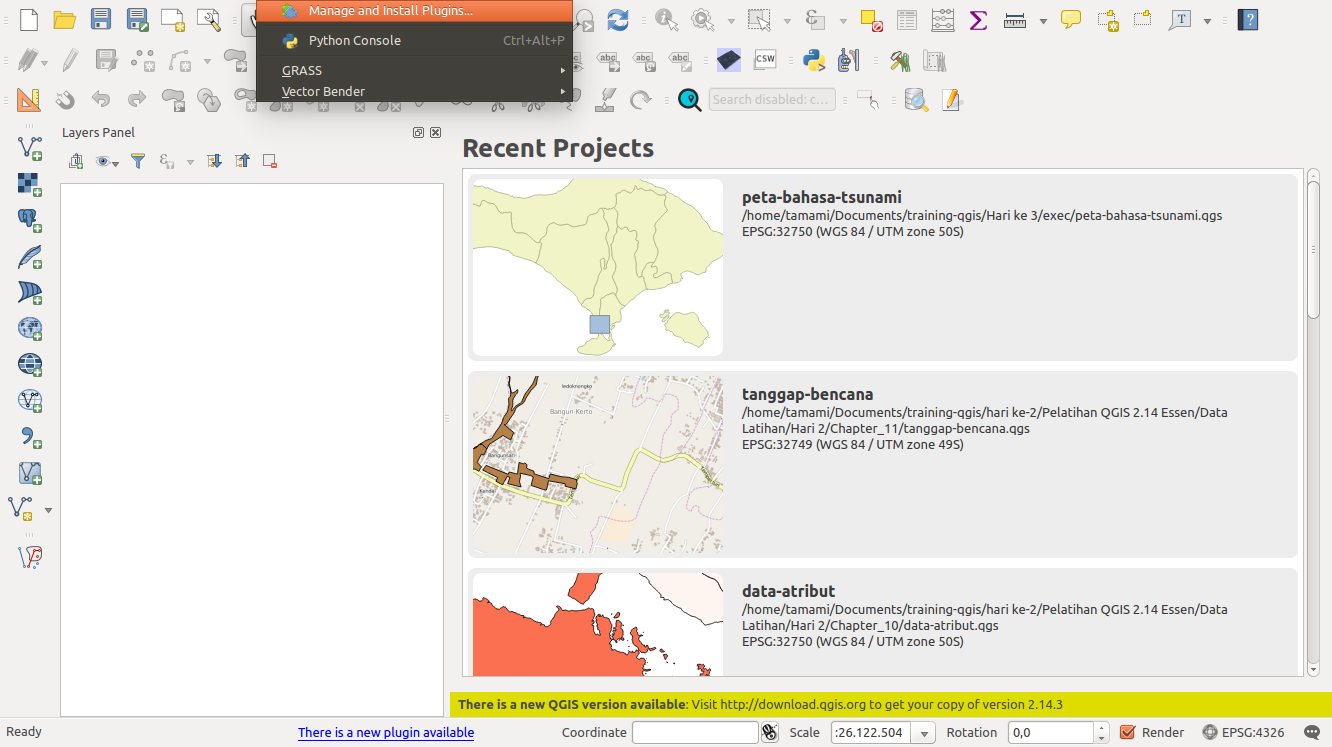
\includegraphics[width=1\textwidth]{./resources/001-manage-plugins-menu}
    \caption{Menu \textit{Manage Plugins}}
    \label{fig:managepluginsmenu}
  \end{figure}
  
  \item Kemudian ketik kata kunci \texttt{OSM} di bagian \textit{search} pada kotak dialog dibagian atas dan pilih komponen seperti pada gambar \ref{fig:osminstallwin}
  
  \begin{figure}[H]
    \centering
    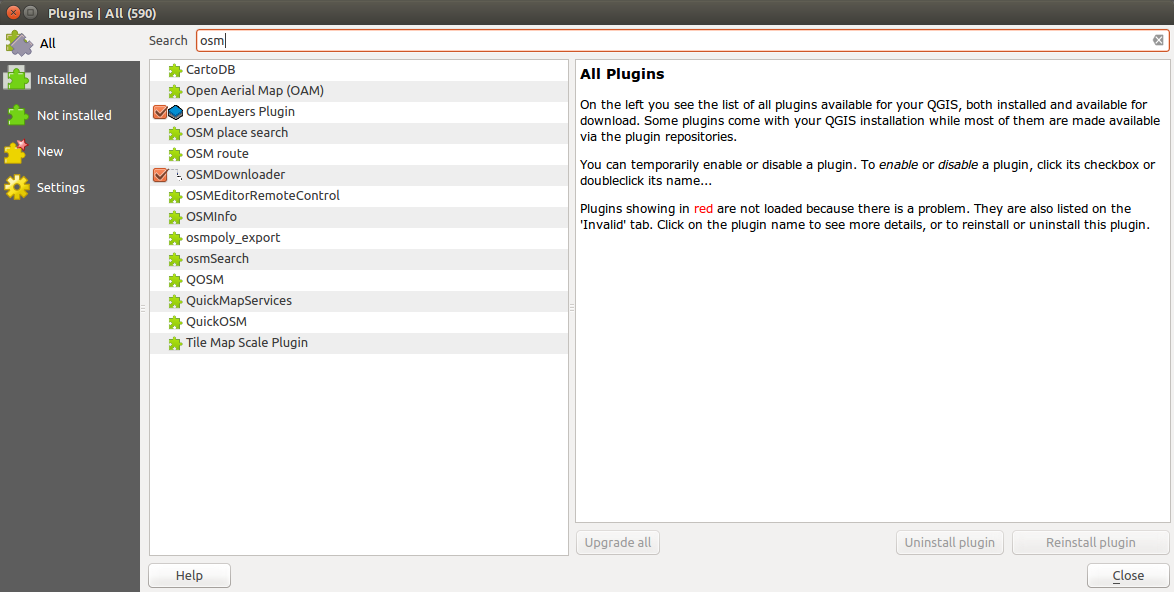
\includegraphics[width=1\textwidth]{./resources/002-osm-install-win}
    \caption{Jendela \textit{Manage Plugins}}
    \label{fig:osminstallwin}
  \end{figure}
\end{enumerate}